

% ЗАМЕТКИ:
%     Гетерогенные инстурменты на основе этой статьи https://sci-hub.se/10.1016/s0304-4076(02)00201-4
    
%     ОЧЕНЬ ХОРОШАЯ СТАТЬЯ, объясняет почему LATE оценка получается с инстурментами и как из нее ATE сделать https://sci-hub.se/https://www.cambridge.org/core/journals/political-analysis/article/beyond-late-estimation-of-the-average-treatment-effect-with-an-instrumental-variable/604E0803793175CF88329DB34DAA80B3
    
%     Вот тут статья обсуждает предопсылку монотонности в более общем случае, а не в бинарном. Но бинарный случай надо рассказать очень хорошо! https://faculty.smu.edu/millimet/classes/eco7377/papers/manski%20pepper%2000.pdf

% \section{Инструментальные переменные -- продолжение}

% \begin{frame}{Late or ATE}
% \begin{itemize}
%     \item 1
%     \item 2
%     \item 3
% \end{itemize}
% \end{frame}

% \begin{frame}{Continuous Instrument}
% \begin{itemize}
%     \item 1
%     \item 2
%     \item 3
% \end{itemize}
% \end{frame}

\section{Четкая разрывная регрессия}

\begin{frame}{Пример}
    \begin{figure}
        \centering
        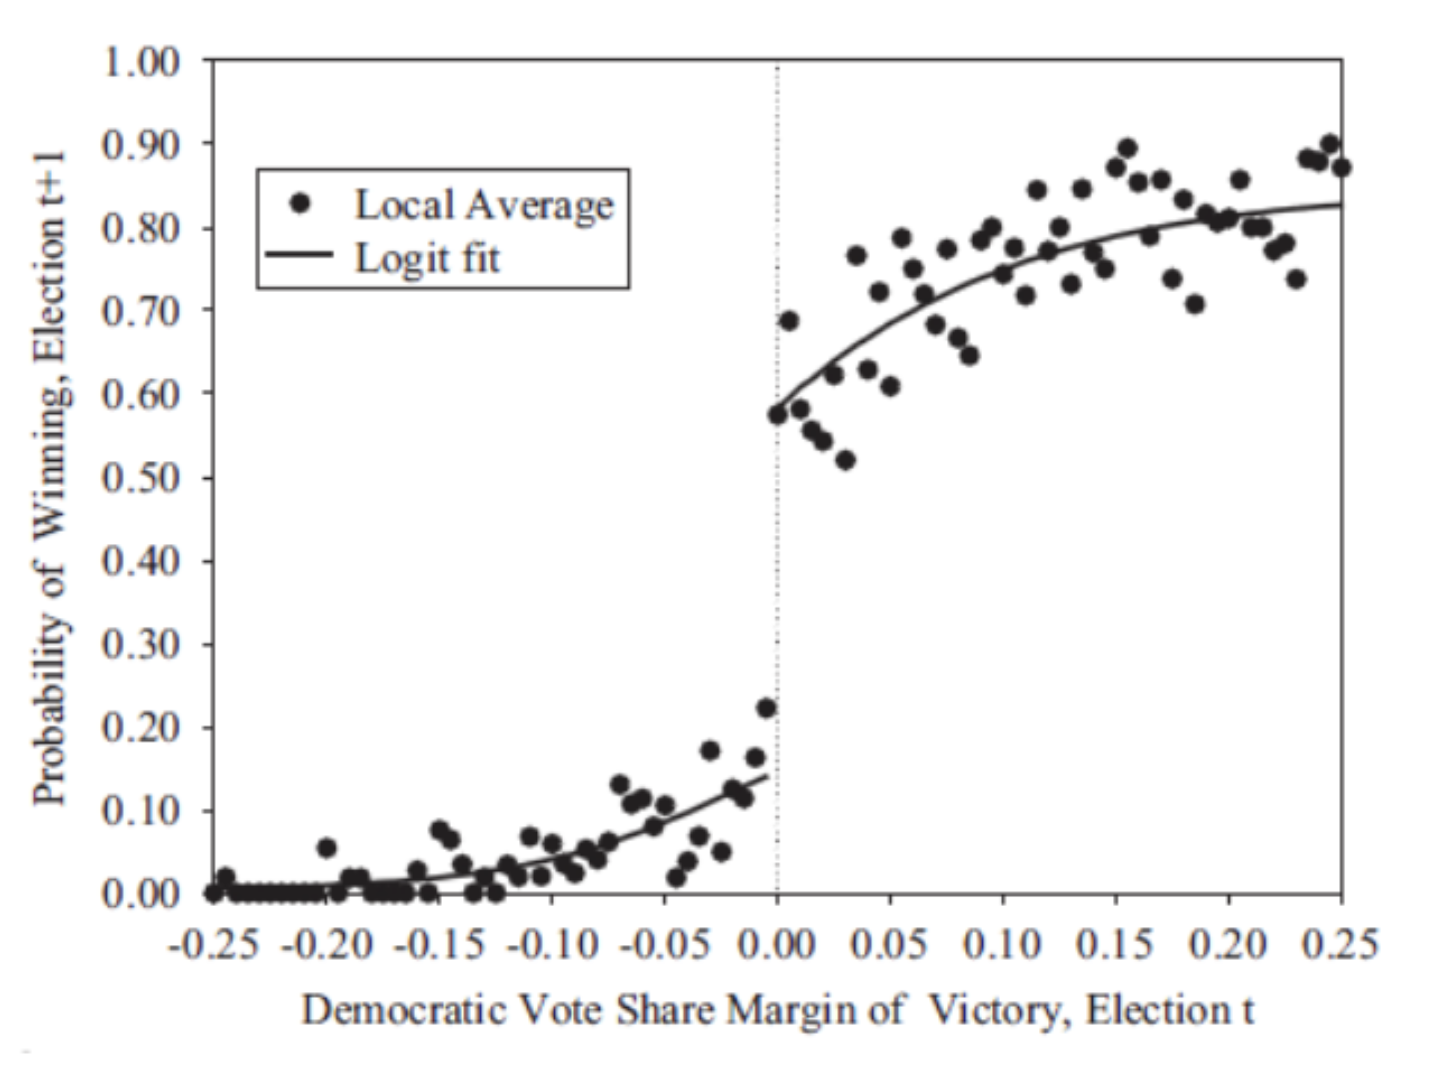
\includegraphics[width=\textwidth]{Lecture_Sources/Images/rdd_votes.png}
    \end{figure}
\end{frame}

\begin{frame}{Еще примеры}

\begin{itemize}
    \item Оценка эффекта образования на будущий доход
    \item Эффект избрания оппозиции на экономику региона
\end{itemize}

\end{frame}


\begin{frame}{Четкая разрывная регрессия: Обозначения}
    \begin{figure}
        \centering
        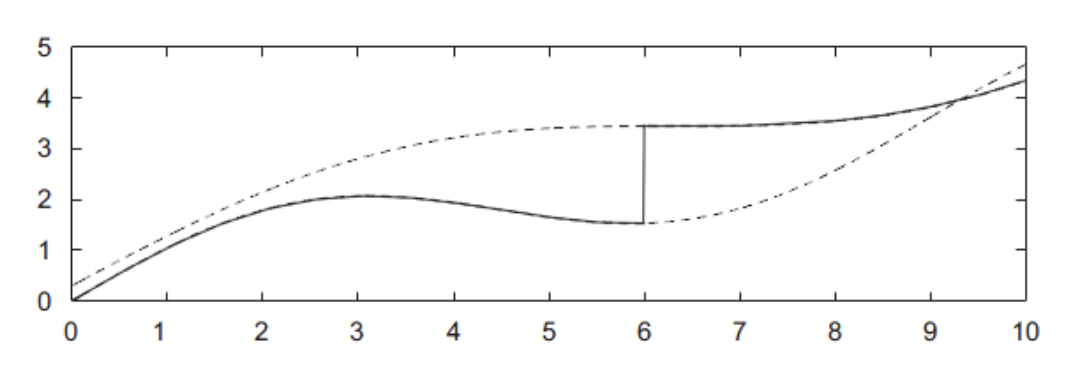
\includegraphics[width=\textwidth]{Images/sharp.png}
    \end{figure}
    \begin{itemize}
        \item Потенциальные исходы $Y_0$, $Y_1$. Ковариаты: $X$
        \item $R$ -- Running variable. По ней проходит граница
        \item $T = \mathbb{I}(R > c)$. $c$ -- отсечка (cutoff)
        \item $Y = TY_1 + (1-T)Y_0$ -- наблюдаемый исход
    \end{itemize}
\end{frame}

\begin{frame}{Четкая разрывная регрессия: Предположения}
    \begin{figure}
        \centering
        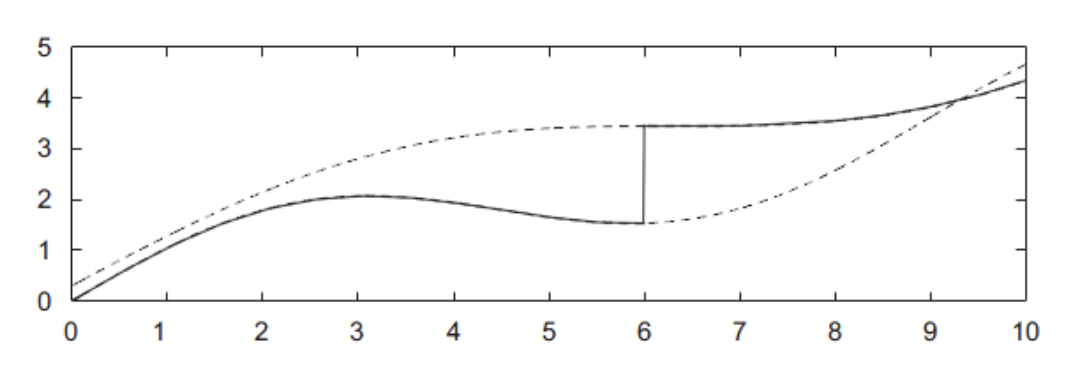
\includegraphics[width=\textwidth]{Images/sharp.png}
    \end{figure}
    Для начала упражнение:
    \begin{itemize}[<+->]
    \item $(Y_0, Y_1, R) \perp T$ -- экзогенность. Выполнена ли? \visible<2->{ \textbf{нет}}
        \item $(Y_0, Y_1) \perp T | R$ -- unconfoundedness. Выполнена ли? \visible<3->{ \textbf{да}}
        \item $1 > P(T | R) > 0$ -- overlap. Выполнена ли? \visible<4->{ \textbf{нет}}
    \end{itemize}
    \pause
    Предположим непрерывность $E(Y_1|R), E(Y_0|R), E(X|R)$ вместо независмости $T$ и $(Y_0, Y_1)$
\end{frame}


\begin{frame}{Четкая разрывная регрессия: оценка}

\begin{itemize}
    \item Выбираем ширину окна h
    \item Берем данные $R \in \left[c-h, c+h\right]$
    \item Оцениваем
\end{itemize}
    % $$
    % \hat Y_{\text{rdd}} = \arg\min_Y \sum^N_i K\left(\frac{||x - x_i||}{h}\right) ((Y_i - Y) T - (Y_i - Y) (1 - T))^2
    % $$
    
    % Или:
    % \begin{gather*}
    % \hat Y_{\text{rdd}} = \frac{1}{\sum(R < 0)}\sum_{R < 0} K\left(\frac{||x - x_i||}{h}\right) Y_i - \\
    % \frac{1}{\sum(R > 0)} \sum_{R > 0} K\left(\frac{||x - x_i||}{h}\right) Y_i
    % \end{gather*}
    
    % простая версия
    \begin{gather*}
    \hat \tau_{\text{rdd}} = \frac{1}{\sum(c - h < R < c)}\sum_{c - h < R < c} Y_i - \\
    \frac{1}{\sum(c + h > R > c)} \sum_{c + h > R > c} Y_i
    \end{gather*}
    
    Или с помощью регрессии:
    
    \begin{gather*}
    Y = a + \tau T
    \end{gather*}
    
    \begin{itemize}
        \item Таким образом мы получаем локальный эффект ($\text{LATE} = \mathbb{E}(\tau|R = c)$)
        % повторить на картинке
    \end{itemize}
\end{frame}



% \begin{frame}{Четкая разрывная регрессия: асимптотика}
% %need theoretical results here
% \end{frame}

\begin{frame}{Контроль на тренд}

\begin{figure}
        \centering
        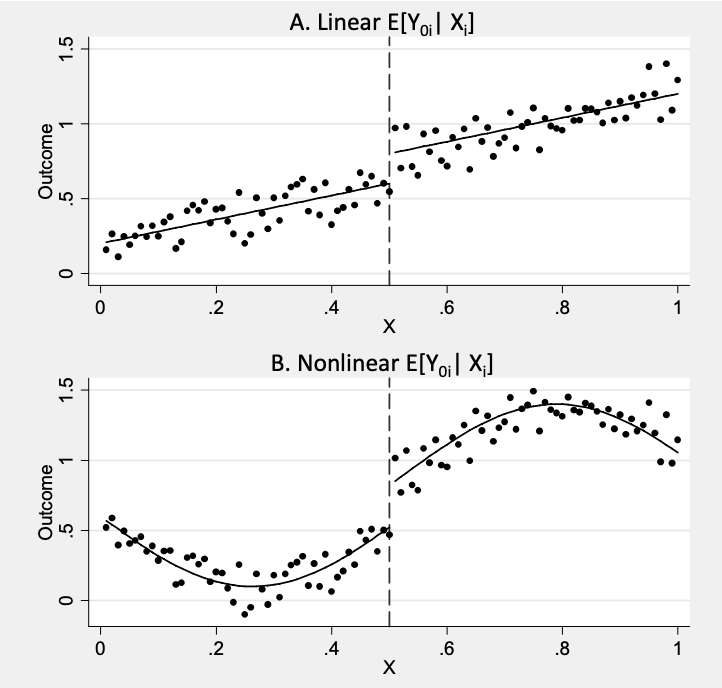
\includegraphics[width=0.6\textwidth]{Lecture_Sources/Images/rdd_trend_control.png}
    \end{figure}

\begin{gather*}
    Y = a_1 + \tau T + a_2 (R - c) + a_3 T (R - c)
\end{gather*}
    
\end{frame}

\begin{frame}{Проверка предположения непрерывности}
    \begin{enumerate}
        \item Проверить непрерывность $Y_1, Y_0$ мы не можем
        \item Но можем проверить непрерывность $X$
    \end{enumerate}
    \begin{figure}
        \centering
        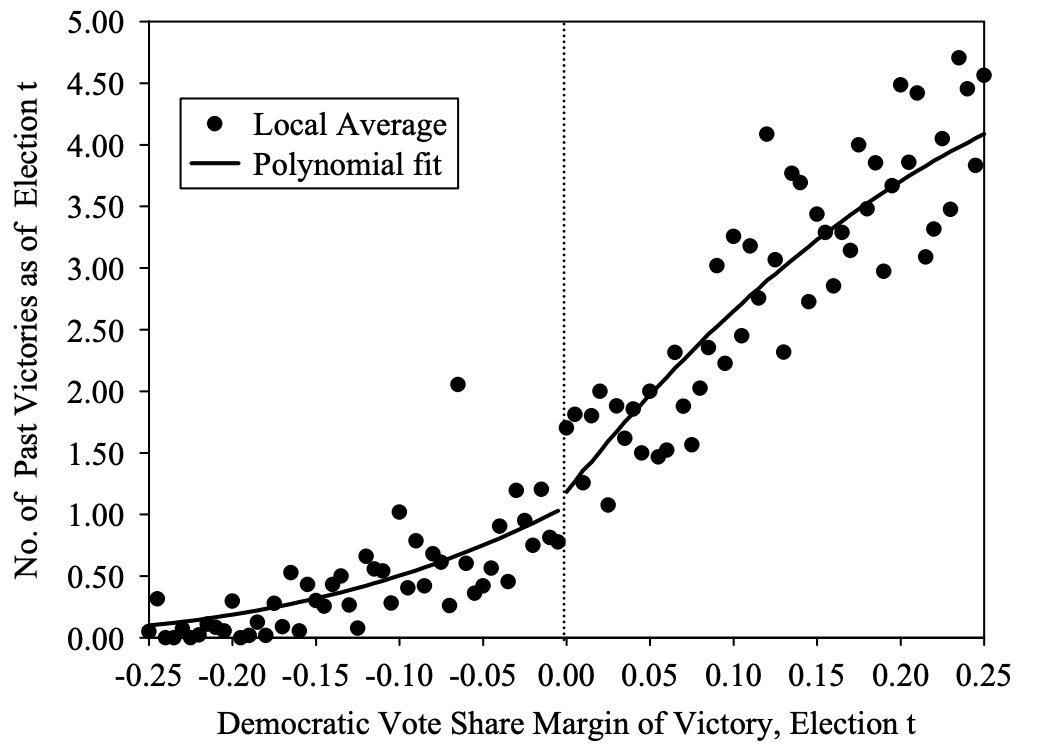
\includegraphics[width=0.8\textwidth]{Images/rdd_placebo.png}
    \end{figure}
\end{frame}


\begin{frame}{Проверка баланса}
    \begin{enumerate}
        \item Проверить, распределение данных по R
    \end{enumerate}
    \begin{figure}
        \centering
        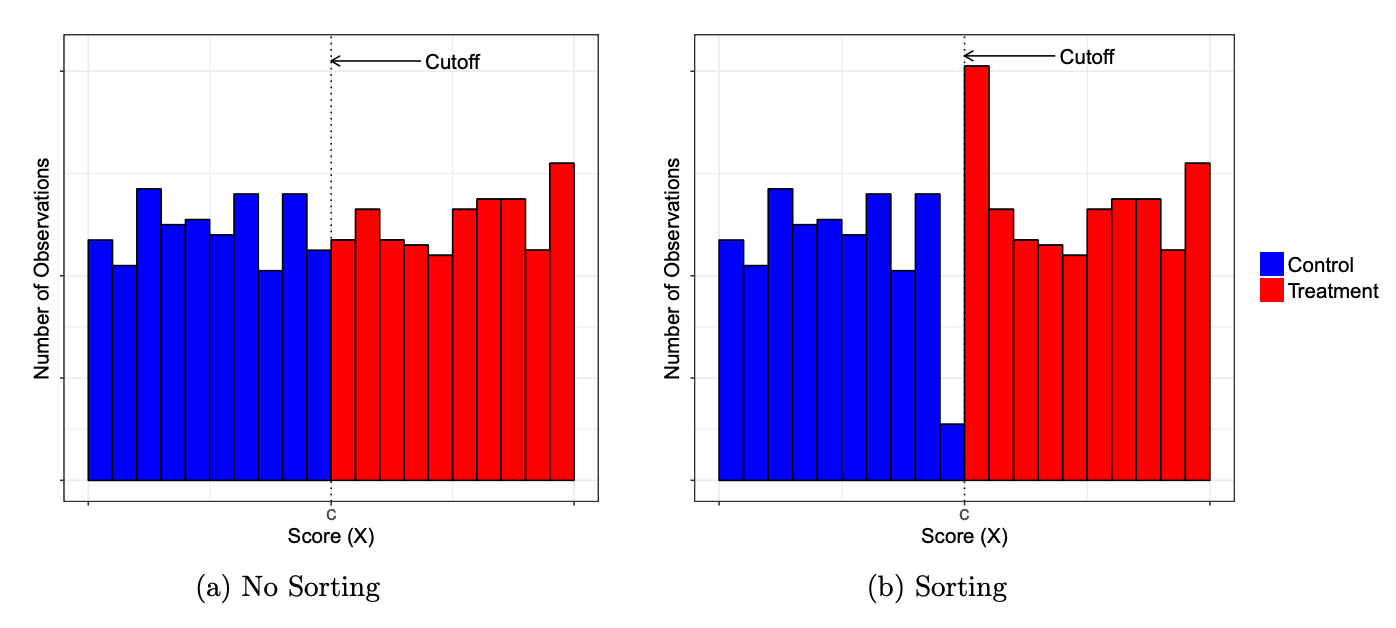
\includegraphics[width=\textwidth]{Images/rdd_density.png}
    \end{figure}
\end{frame}

\begin{frame}{Проверка чувствительности к ширине окне}
    \begin{figure}
        \centering
        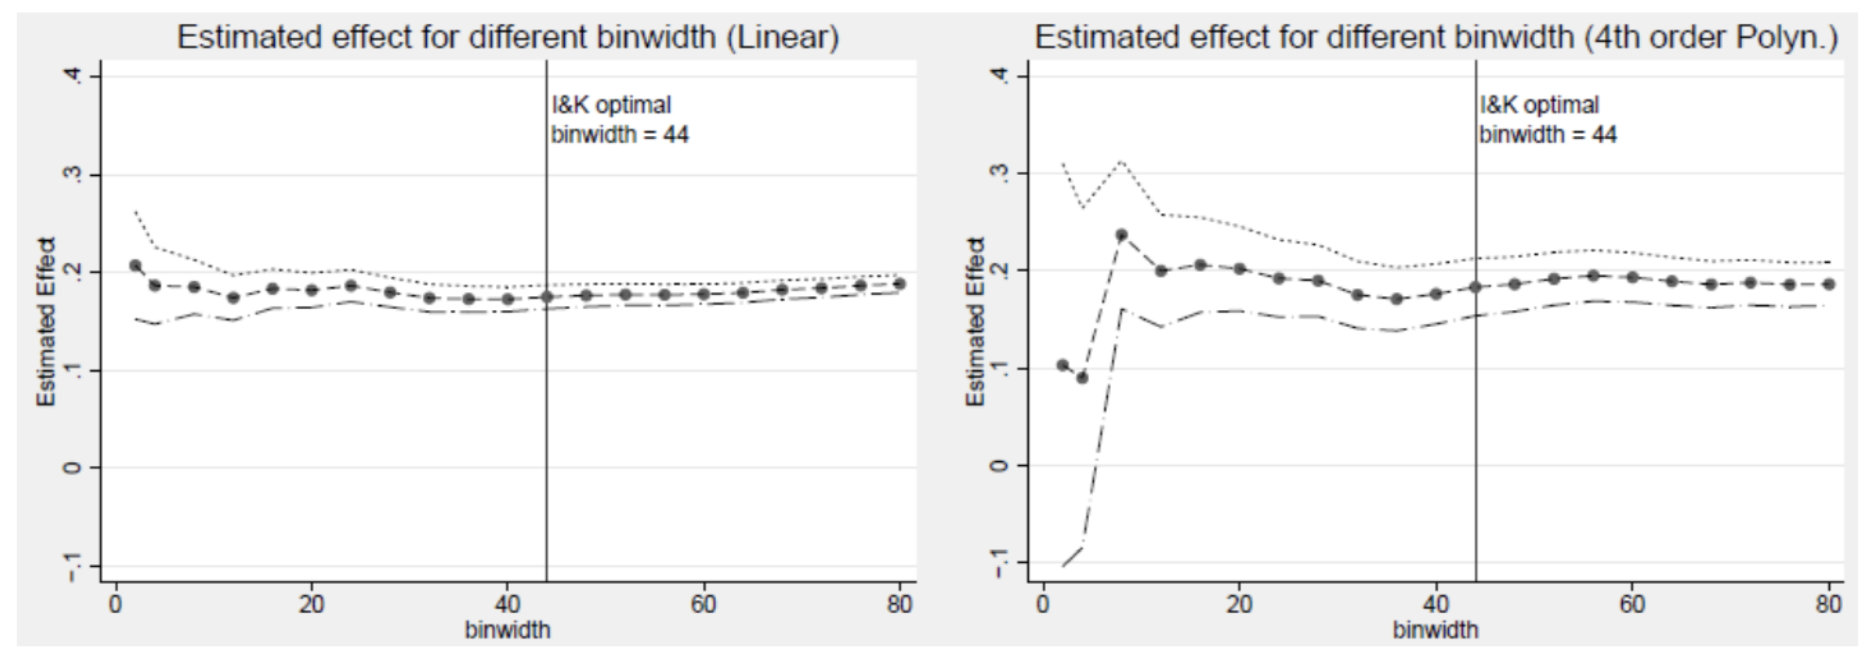
\includegraphics[width=\textwidth]{Images/rdd_sensitivity.png}
    \end{figure}
    Чем меньше окно, тем меньше дисперсия, но больше смещение
\end{frame}

% \begin{frame}{Как выбирать ширину окно?}

% \end{frame}


\begin{frame}{Есть ли смысл контролировать на другие переменные в этой регрессии?}
\begin{itemize}
    \item Не для того, чтобы избавиться от смещения
    \item Для того, чтобы снизить дисперсию
\end{itemize}
\end{frame}

